\documentclass[letterpaper]{article}
\usepackage[margin=1in]{geometry}
\usepackage[utf8]{inputenc}
\usepackage{textcomp}
\usepackage{amssymb}
\usepackage{natbib}
\usepackage{graphicx}
\usepackage{gensymb}
\usepackage{amsthm, amsmath, mathtools}
\usepackage[dvipsnames]{xcolor}
\usepackage{enumerate}
\usepackage{mdframed}
\usepackage[most]{tcolorbox}
\usepackage{csquotes}
% https://tex.stackexchange.com/questions/13506/how-to-continue-the-framed-text-box-on-multiple-pages

\tcbuselibrary{theorems}

\newcommand{\R}{\mathbb{R}}
\newcommand{\Z}{\mathbb{Z}}
\newcommand{\N}{\mathbb{N}}
\newcommand{\Q}{\mathbb{Q}}
\newcommand{\C}{\mathbb{C}}
\newcommand{\code}[1]{\texttt{#1}}
\newcommand{\mdiamond}{$\diamondsuit$}
\newcommand{\PowerSet}{\mathcal{P}}
\newcommand{\Mod}[1]{\ (\mathrm{mod}\ #1)}
\DeclareMathOperator{\lcm}{lcm}

%\newtheorem*{theorem}{Theorem}
%\newtheorem*{definition}{Definition}
%\newtheorem*{corollary}{Corollary}
%\newtheorem*{lemma}{Lemma}
\newtheorem*{proposition}{Proposition}


\newtcbtheorem[number within=section]{theorem}{Theorem}
{colback=green!5,colframe=green!35!black,fonttitle=\bfseries}{th}

\newtcbtheorem[number within=section]{definition}{Definition}
{colback=blue!5,colframe=blue!35!black,fonttitle=\bfseries}{def}

\newtcbtheorem[number within=section]{corollary}{Corollary}
{colback=yellow!5,colframe=yellow!35!black,fonttitle=\bfseries}{cor}

\newtcbtheorem[number within=section]{lemma}{Lemma}
{colback=red!5,colframe=red!35!black,fonttitle=\bfseries}{lem}

\newtcbtheorem[number within=section]{example}{Example}
{colback=white!5,colframe=white!35!black,fonttitle=\bfseries}{def}

\newtcbtheorem[number within=section]{note}{Important Note}{
        enhanced,
        sharp corners,
        attach boxed title to top left={
            xshift=-1mm,
            yshift=-5mm,
            yshifttext=-1mm
        },
        top=1.5em,
        colback=white,
        colframe=black,
        fonttitle=\bfseries,
        boxed title style={
            sharp corners,
            size=small,
            colback=red!75!black,
            colframe=red!75!black,
        } 
    }{impnote}
\usepackage[utf8]{inputenc}
\usepackage[english]{babel}
\usepackage{fancyhdr}
\usepackage[hidelinks]{hyperref}

\pagestyle{fancy}
\fancyhf{}
\rhead{Math 170B}
\chead{Wednesday, May 10, 2023}
\lhead{Lecture 17}
\rfoot{\thepage}

\setlength{\parindent}{0pt}

\begin{document}

\section{Basis Spline (Section 6.5)}
The idea is that we'll have \emph{limitless} knots. So, for the knots $t_i$ such that $i \in \Z$ and \[\hdots < t_i < t_{i + 1} < \hdots,\] $B_{i}^{k}(x)$ is a degree $k$, $i$th B-Spline. 

\subsection{0th Degree B-Spline}
\begin{mdframed}
    (Example.) For $k = 0$, we have 
    \[B_{i}^{0}(x) = \begin{cases}
        1 & t_{i} \leq x < t_{i + 1} \\ 
        0 & \text{otherwise}
    \end{cases}.\]

    \begin{center}
        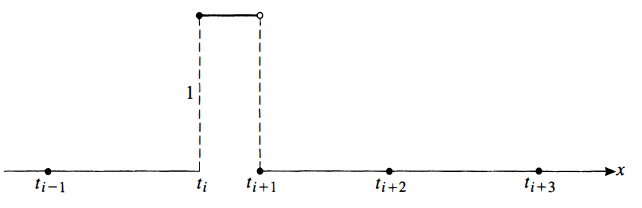
\includegraphics[scale=0.8]{../assets/bspline_1.png}
    \end{center}
\end{mdframed}

Let's now consider the following sequence of 0th degree B-splines, 
\[\{B_{i}^0, i \in \Z\}.\]
Some properties of this sequence include 
\begin{itemize}
    \item \textbf{Support} ($B_{i}^0 (x) \neq 0$) is $[t_i, t_{i + 1})$. 
    \item $B_{i}^0 \geq 0$ for all possible $x$ and all possible $i$.
    \item Continuous from right. 
    \item For all $x$, $\sum_{i = -\infty}^{\infty} B_{i}^{0}(x) = 1.$
\end{itemize}
For given knots, $B_{i}^0$ is a basis for all degree zero splines.

\begin{mdframed}
    (Example.) Let $S(x) = c_i$ for $t_{i} \leq x < t_{i + 1}$ and $i \in \Z$, we have 

    \begin{center}
        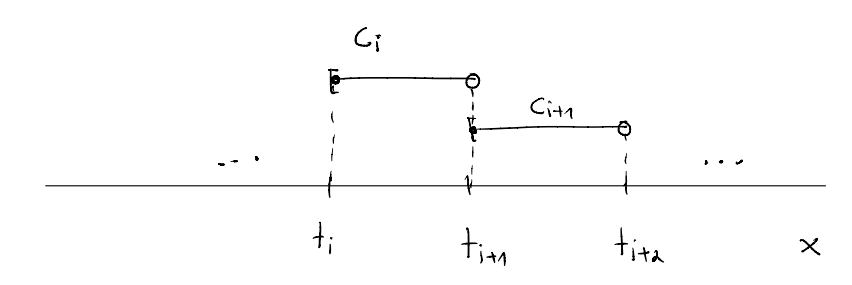
\includegraphics[scale=0.5]{../assets/bspline_2.png}
    \end{center}

    Then, we can say that 
    \[S(x) = \sum_{i = -\infty}^{\infty} c_{i} B_{i}^{0}(x).\]
\end{mdframed}

\subsection{Higher Degree B-Splines}
We can make use of the following recursion to construct higher degree B-splines: 
\[B_{i}^{k}(x) = \left(\frac{x - t_i}{t_{i + k} - t_{i}}\right)B_{i}^{k - 1}(x) + \left(\frac{t_{i + k + 1} - x}{t_{i + k + 1} - t_{i + 1}}\right) B_{i + 1}^{k - 1}(x)\]
\[V_{i}^{k}(x) = \frac{x - t_{i}}{t_{i + k} - t_i},\]
meaning we can rewrite the above $B_{i}^{k}$ as
\[B_{i}^{k} = V_{i}^{k} B_{i}^{k - 1} + (1 - V_{i + 1}^{k}) B_{i + 1}^{k - 1}.\]


\begin{mdframed}[nobreak=true]
    (Example.) To find the degree 1 B-spline, we can write 
    \[B_{i}^{1} = V_{i}^{1} B_{i}^{0} + (1 - V_{i + 1}^{1}) B_{i + 1}^{0} = \begin{cases}
        0 & x < t_i \text{ or } x \geq t_{i + 2} \\ 
        V_{i}^{1} & t_i \leq x < t_{i + 1} \\ 
        (1 - V_{i + 1}^{1}) & t_{i + 1} \leq x < t_{i + 2} \\ 
    \end{cases}.\]
\end{mdframed}
What are some properties of the degree 1 B-spline? 
\begin{itemize}
    \item Support: $x \in (t_{i}, t_{i + 2})$.
    \item $B_{i}^{1}(x) \geq 0$ for all $i$ and $x$.
    \item Continuous and differentiable except at the knots themselves (i.e, $t_{i}, t_{i + 1}, t_{i + 2}$).
    \item For all $x$, 
    \[\sum_{i = \infty}^{\infty} B_{i}^{1}(x) = 1.\]
    In particular, for any $x$, we can find an interval $t_{j} \leq x < t_{j + 1}$. Then, $B_{j - 1}^{1}$ and $B_{j}^{1}$ are the only non-zero B-splines:
    \[B_{j - 1}^{1}(x) = \frac{t_{j + k} - x}{t_{j + k} - t_j} = 1 - V_{j}^{1}.\]
    \[B_{j}^{k} = \frac{x - t_j}{x_{j + k} - t_j} = V_{j}^{1}.\]
    \[B_{j - 1}^{1} + B_{j}^{1} = (1 - V_j^{1}) + V_j^1 = 1.\]
\end{itemize}

\subsection{Algorithm to Generate Higher Degree B-Spline}
Using the recursion defined above, in particular with $t$ being defined as 
\[t = \{t_i, t_{i + 1}, t_{i + 2}, \hdots, t_{i + 1 + k}\},\]
we have the following algorithm:
\begin{algorithm}[H]
    \caption{Higher Degree B-Spline}
    \begin{algorithmic}[1]
        \Function{BSpline}{$x, k, i, t$}
            \If{$1 \leq k$}
                \State $V_{i} \gets \frac{x - t_i}{t_{i + k} - t_i}$
                \State $V_{i + 1} \gets \frac{t_{i + k + 1} - x}{t_{i + k + 1} - t_{i + 1}}$
                \State $B_{i}^{k} = V_{i} \cdot \text{BSpline}(x, k - 1, i, t) + (1 - V_{i + 1}) \cdot \text{BSpline}(x, k - 1, i + 1, t)$
            \Else \Comment{If $k = 0$ (base case)}
                \If{$t_i \leq x$ and $x < t_{i + 1}$}
                    \State $B_{i}^{k} \gets 1$
                \Else 
                    \State $B_{i}^{k} \gets 0$
                \EndIf  
            \EndIf 
        \EndFunction 
    \end{algorithmic}
\end{algorithm}
% outputs B_{i}^{k}(x)


\end{document}